%   MSc Business Analytics Dissertation
%
%   Title:     Aaa Bbbbbbb Cccccccccc
%   Author(s): Xxxxxx Xxxxxxxxx and Yyy Yyyyyyyyy
%
%   Chapter 5: Results
%
%   Change Control:
%   When     Who   Ver  What
%   -------  ----  ---  --------------------------------------------------------------
%   11Feb11  AB    0.1  Begun 
%

\chapter{Results}\label{C.Results}

\section{Overview}
Model prediction accuracy of original test data set was 99.65\%, which is practically impossible. As discussed in chapter \ref{C.intro} actual data received from KPMG was made up using pre-defined formulas and rules to make it look real. Data didn't cover all possible scenario for a loan portfolio and achieving an accuracy of 99\% in credit scoring model is difficult as one needs to train model recursively with large data size covering all permutations and combinations of situations for loan default.


\section{Introduction}\label{S.intro5}

Original data set consist of 237389 observations and 35 variables, according to data 95\% loan applications will not default, and only 5\% application had chances to default. Therefore, to consider all possible scenarios data has been modified and a data subset has been generated from original dataset to carry experiments. New dataset has 36696 observations and 26 variabls. 

\begin{table}[]
\centering
\caption{Comparison of Logistic Regression and Decision Tree performance}
\label{table:results}
\begin{tabular}{@{}lccc@{}}
\toprule
\textbf{Model}               & \textbf{AUROC} & \textbf{KS} & \textbf{Gini} \\ \midrule
\textbf{Logistic Regression} & 68.34          & 13.53       & 36.68         \\
\textbf{Decision Tree}       & 81.11          & 60.04       & 62.22         \\ \bottomrule
\end{tabular}
\end{table}


\begin{center}
\begin{figure}[!htb]
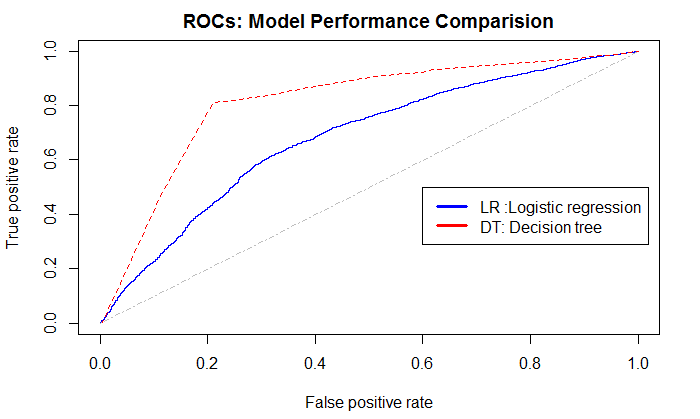
\includegraphics[width=\textwidth]{results1.png}
\centering
\caption{ROCs for logistic regression vs decision tree}{\textbf{Source:} Plotted in R Studio}
\label{fig:result}
\end{figure}
\end{center}

In table. \ref{table:results}, KS is the Kolmogorov-Smirnov goodness-of-Fit Test (or KS-Test), GINI is Gini coefficient of inequality distribution of response variable and AUC is Area under ROC (Receiver Operating Chaterstics) curve.


Receiver under curve is one of technique to estimate the performance of predictive model.

Limitations of data in real life application. Accuracy might vary

As provided was made up due to confidential agreement. Data is generated from pre-defined formulas which made it look quite original but it could cover all possible scenarios of real life. For example, it failed to consider a scenario when a customer is defaulting while being in creting rating 1 (Good Credit). \\

Intially, Logistic Regression and Decsion tree were giving accuracy of 99.31\% which is practially not possible in credit scoring. during this research work we found that various other researchers also pointed out that Logistic regression is much better modelling technique than any other statsical techqnique. For Instance Mr.x noted in work that neural network can work at par with logistic regression model provided that the target variable is predict result in yes or no.\\

Similarly decision tree has other limitations with respect to number of possible nodes and leafs for making creteria. hence decision tree end with less number of rules. Mr. Y compared the performance of Decesion tree and LR and found LR performance is higher than 5\%

As per dasssssssssssh paper 25 - 30\% error is expected in credit rating system because human nature is quite difficult to predict. Similar in this scenario it is quite complex to various parameter to consider to build solid system which have high accuracy. One of the leading bank in Ireland in past attempted to consider upto 600 parameter to all possible cases of credit using Artificial Intelligence 
testiing of model.

Accuracy reduced to 25\% after scaling variables. Compare difference between model performance and how it is improved.

How we implemented the model

Explaing Limitations of Algorithm and why one algo is better
FUTURE SCOPE IS AI of this credit scoring


